\documentclass{article}
\usepackage[paperwidth=3.25in,paperheight=1.75in,margin=0.08in]{geometry}
\usepackage[T1]{fontenc}
\usepackage{lmodern,tikz,xcolor}
\usetikzlibrary{arrows.meta,positioning}
\definecolor{teal}{HTML}{007F86}
\definecolor{pale}{HTML}{EDF4F3}
\pagestyle{empty}
\setlength{\parindent}{0pt}
\begin{document}
\centering
{\sffamily\bfseries\fontsize{9}{10}\selectfont From molecules to polymer grafts}\par\vspace{7pt}
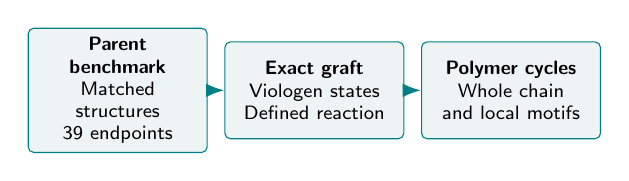
\begin{tikzpicture}[>=Latex,node distance=6pt,every node/.style={font=\sffamily\fontsize{7}{8}\selectfont,align=center}]
\node[draw=teal,fill=pale,rounded corners=2pt,text width=58pt,minimum height=35pt] (a) {\textbf{Parent benchmark}\\Matched structures\\39 endpoints};
\node[draw=teal,fill=pale,rounded corners=2pt,text width=58pt,minimum height=35pt,right=of a] (b) {\textbf{Exact graft}\\Viologen states\\Defined reaction};
\node[draw=teal,fill=pale,rounded corners=2pt,text width=58pt,minimum height=35pt,right=of b] (c) {\textbf{Polymer cycles}\\Whole chain\\and local motifs};
\draw[->,teal,thick] (a)--(b);\draw[->,teal,thick] (b)--(c);
\end{tikzpicture}\par\vspace{7pt}
{\sffamily\fontsize{7.5}{9}\selectfont Fc cancels from paired redox-step spacings.\par
Whole-chain response differs from motif interaction.}\par\vspace{4pt}
{\sffamily\fontsize{6.5}{8}\selectfont Molecular validation and finite polymer comparisons}
\end{document}
